\documentclass[a4paper, 12pt, twoside]{article}
\usepackage[T2A,T1]{fontenc}
\usepackage[utf8]{inputenc}
\usepackage[english, russian]{babel}
\usepackage{graphicx}
\usepackage[hcentering, bindingoffset = 10mm, right = 15 mm, left = 15 mm, top=20mm, bottom = 20 mm]{geometry}
\usepackage{multirow}
\usepackage{ctable}
\usepackage{lipsum}
\usepackage{amsmath, amstext}
\usepackage{siunitx}
\usepackage{subcaption}
\usepackage{wrapfig}
\usepackage{adjustbox}
\usepackage{enumerate, indentfirst, float}
\usepackage{capt-of, svg}
\usepackage{cmap} % Улучшенный поиск русских слов в полученном pdf-файле
\usepackage{comment}
\graphicspath{{pictures/}} 
\usepackage{multicol}
% \usepackage{alltt}
\usepackage{verbatim}
\usepackage[colorlinks,urlcolor=blue]{hyperref}
\usepackage{tocvsec2}

%\usepackage{pscyr} % Нормальные шрифты
\usepackage[normalem]{ulem} % для подчёркиваний uline
\ULdepth = 0.16em
%% Перенос знаков в формулах (по Львовскому)
\newcommand*{\hm}[1]{#1\nobreak\discretionary{}
	{\hbox{$\mathsurround=0pt #1$}}{}}

\usepackage{fancyhdr} %Колонтикулы
\pagestyle{fancy}
\lhead{
\includegraphics[width = 10 mm]{logo.jpg} 3D-scanner}
% \rhead{\textit{\today}}
\rhead{\textit{25 марта 2022 г.}}

\newenvironment{bottompar}{\par\vspace*{\fill}}{\clearpage}
 
% \setcounter{secnumdepth}{2}

\begin{document}
\begin{titlepage}

\newcommand{\HRule}{\rule{\linewidth}{0.7mm}} % Defines a new command for the horizontal lines, change thickness here

\center % Center everything on the page
 
%----------------------------------------------------------------------------------------
%	HEADING SECTIONS
%----------------------------------------------------------------------------------------

\textsc{\LARGE Московский Физико-Технический Институт}\\[1,5cm] % Name of your university/college

\textsc{\large Итоговый проект по курсу Донова Г.И. "Микроконтроллеры"} \\[1.0cm] % Minor heading such as course title
\textsc{\LARGE ФРКТ 2022} \\[0.5cm]

%----------------------------------------------------------------------------------------
%	TITLE SECTION
%----------------------------------------------------------------------------------------

\HRule
\\[0.4cm]
{ \huge \bfseries THE 3D-SCANNER}
\\[0.4cm] % Title of your document
\HRule
\\[0.5cm]


 
%----------------------------------------------------------------------------------------
%	AUTHOR SECTION
%----------------------------------------------------------------------------------------


	\begin{center} \large

		\textbf{Авторы:}  \\
		\textit{Группа: Б01-006} \\
		Штундер Арсений
	\end{center}

\begin{figure}[h!]
    \centering
    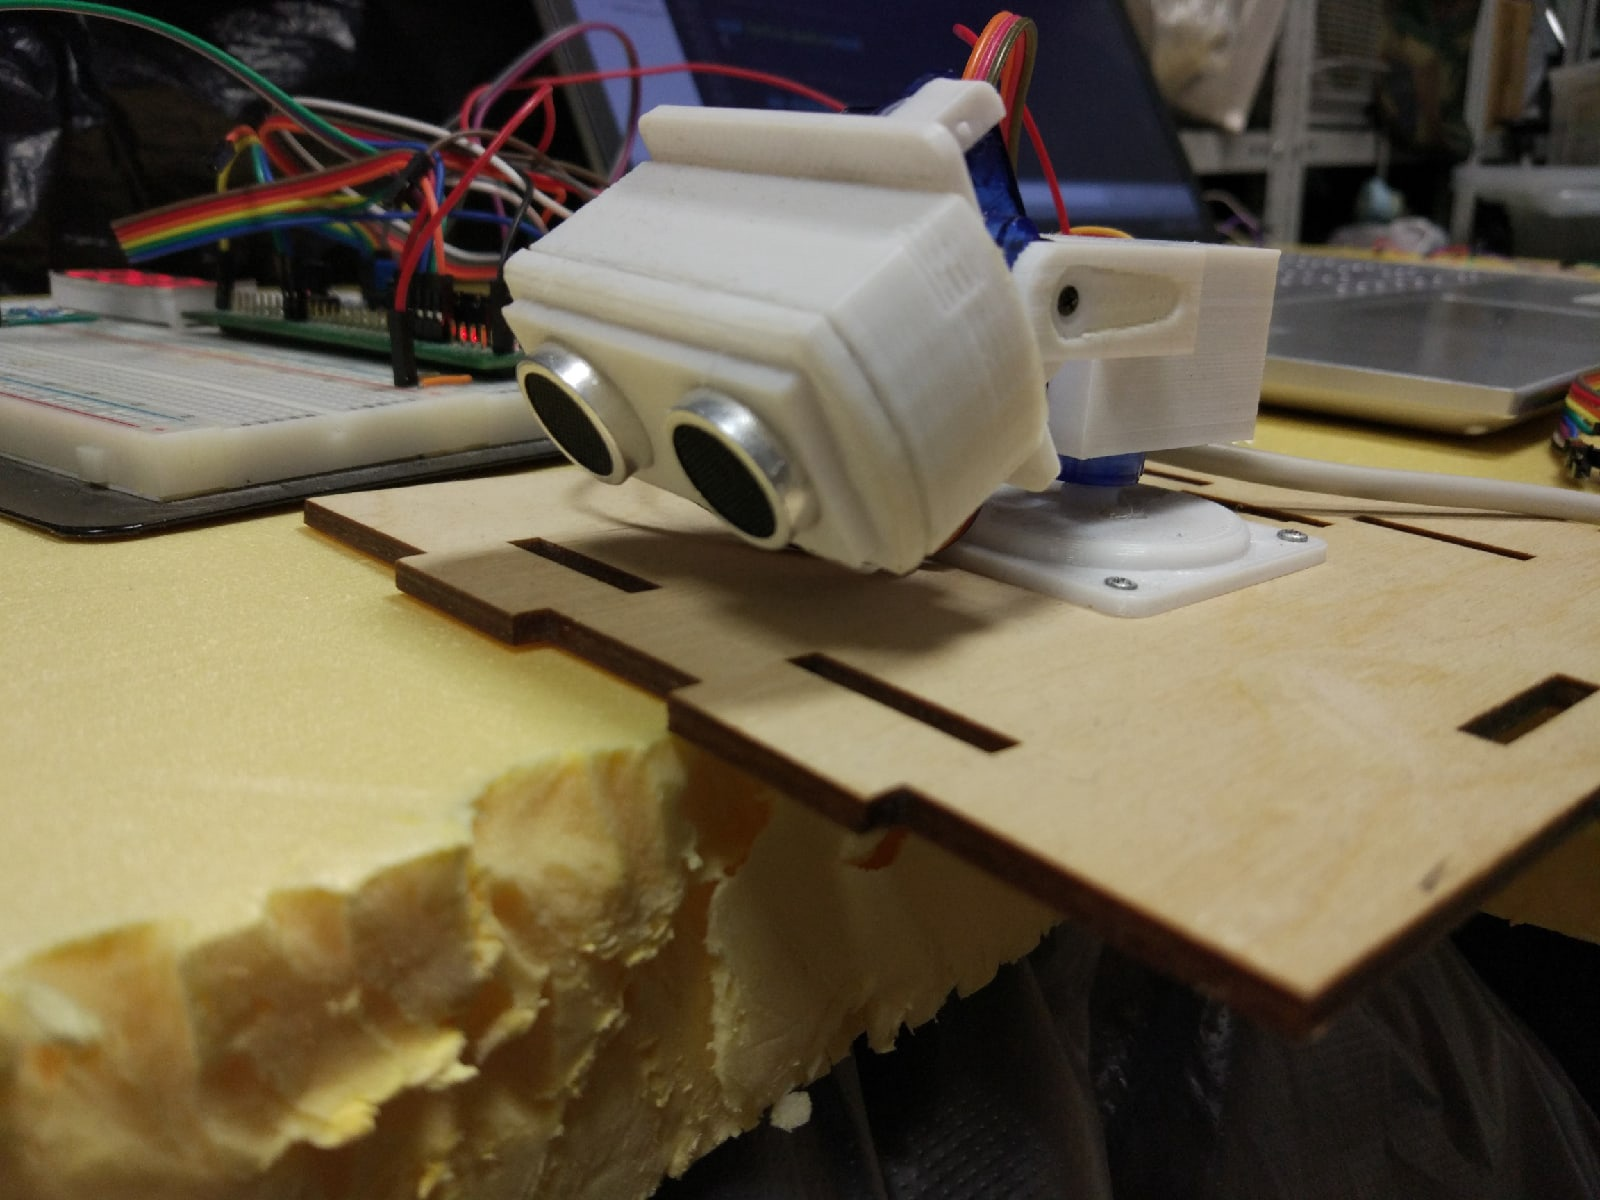
\includegraphics[scale = 0.15]{scan1.jpg}
    %\caption{Фото 3d-сканера}
\end{figure}

~


\begin{bottompar}
	\begin{center}
		
\includegraphics[width = 80 mm]{logo.jpg}
	\end{center}
	{\large Долгопрудный, 25 марта 2022}

\end{bottompar}
\vfill % Fill the rest of the page with whitespace

\end{titlepage}

\section*{Цель работы:}
Научиться сканировать пространство и выводить 3d-график на компьютер.

\section*{Используемое оборудование:}
Микроконтроллер STM32F051R8T6, ультразвуковой датчик HC-SR04, USB-TTL преоброзователь на базе CP2102, 2 сервопривода, соединительные провода, 7-сегментный индикатор, 8 резисторов, макетная плата, ноутбук.    

\section*{Описание проекта:}
Проект сделан на базе микроконтроллера STM32F051R8T6.\\  
В проекте имеется 7-сегментный индикатор, который служит для вывода необходимой информации, такой как приветствие и расстояние в каждый момент времени. Благодаря двум сервоприводам происходит поворот ультразвукового датчика в пространстве, который считывает расстояние до объекта. В каждый момент времени это расстояние выводится на индикатор, а также передается через UART для дальнейшей отрисовки графика. 
\vfill
\begin{figure}[h!]
	\begin{multicols}{2}
	\hfill
	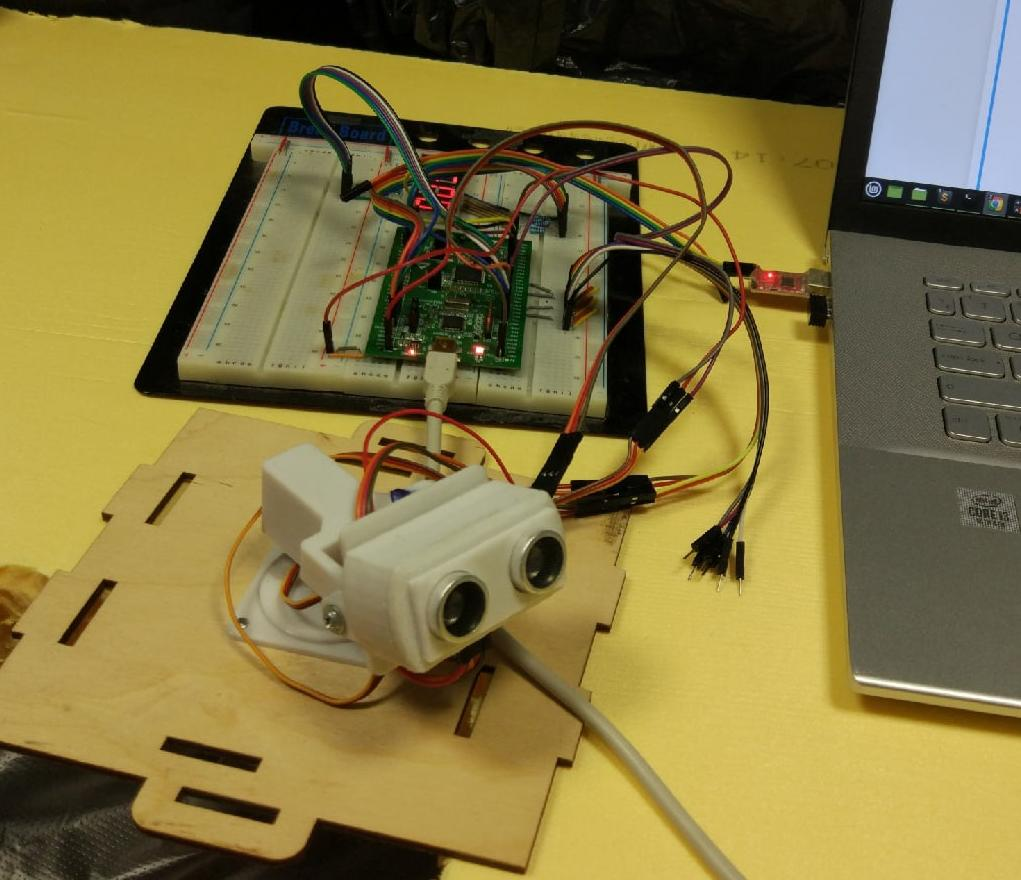
\includegraphics[height=60mm, width=80mm]{scan2.jpg}
	%\vfill
	\caption{3d-сканер}
	\label{figLeft}
	\hfill
	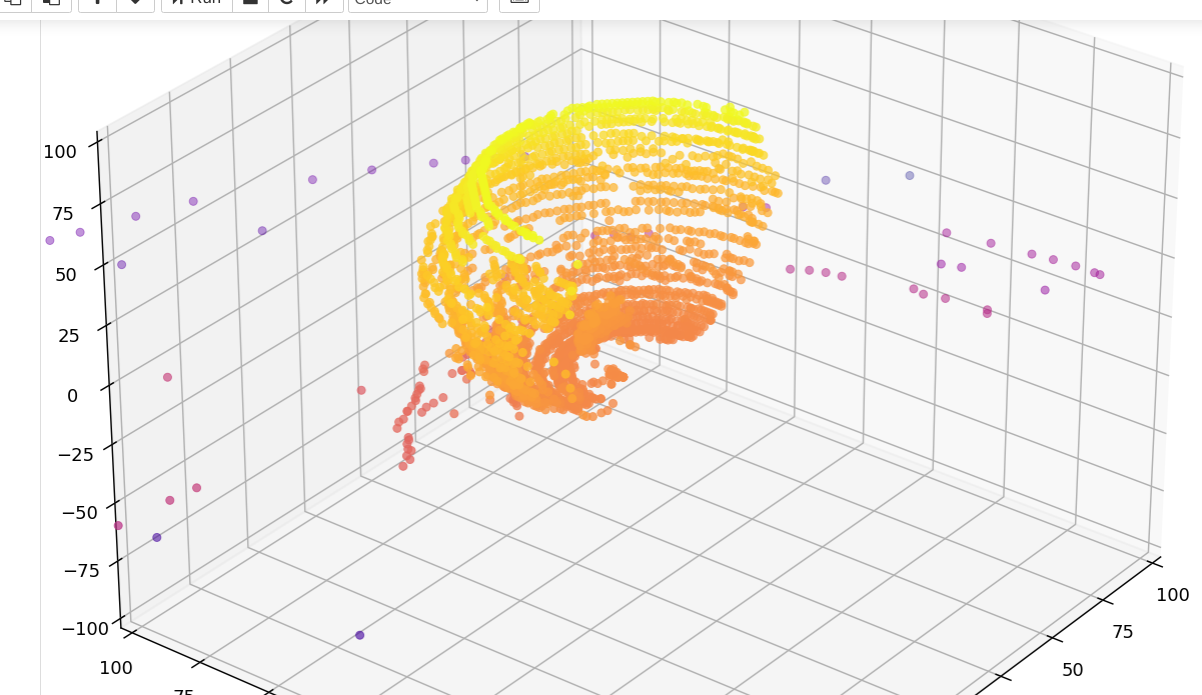
\includegraphics[height=60mm, width=80mm]{graph1.png}
	%\vfill
	\caption{График просканированного пр-ва}
	\label{figRight}
	\end{multicols}
\end{figure}

\section*{Алгоритм работы:}
Изначально происходит инициализация всей переферии, необходимой для дальнейшей работы. \\
\indent Затем работа проекта начинаетя с приветствия на 7-семисегментном индикаторе, который прокручивает текст. Сразу после настраиваются таймеры, для синхронного взаимодействия сервоприводов и вывода расстояние на индикатор, ультразвукового датчика и usb-uart модуля.\\
\indent С помощью Углов Эйлера пересчитываем расстояние до объекта для Декартовой СК(для  вывода графика на ноутбуке). Затем происходит отправка через uart 3-x компонент координат для точки, и так непрерывным потоком для каждой точки происходит отправка. Скрипт, который считывает поток данных, полученных с usb-uart, отрисовывает точки, и получается график просканированного пространства.    

\section*{Исходный код:}
\begin{verbatim}
/* |\/\/\/\/\/\/\/\/\/\/\/\/\/\/\/\/\/\/\/\/\/\/\/\/\/\/\/\/\    |
 * |-------------------------------------------------------------|
 * | It's a CONCLUSION PROJECT in the course of Microcontrollers |
 * |               This is Ultrasonic 3d_scanner                 |
 * |-------------------------------------------------------------|
 * |----------------------THE_MAIN_IDEA--------------------------|
 * |=============================================================|
 * |It scans the space using ultrasonic sensor and two servos    |
 * |Also it shows the distance on the 7-segment indicator        |
 * |and sends it through the usart to show data in graph         |
 * |=============================================================|
 */

#include "stm32f0xx_ll_rcc.h"
#include "stm32f0xx_ll_system.h"
#include "stm32f0xx_ll_bus.h"
#include "stm32f0xx_ll_gpio.h"
#include "stm32f0xx_ll_tim.h"
#include "stm32f0xx_ll_usart.h"

#include "stm32f0xx_ll_exti.h"
#include "stm32f0xx_ll_utils.h"
#include "stm32f0xx_ll_cortex.h"
#include "math.h"

/*---------------------------------------------------------------------*/
/*------------------Some information about servos----------------------*/

/* ========================================================
 * Pulse_duration: 0.5 - 2.6(ms), (normal: 0.6 - 2.4(ms) )
 * Period: 20 ms
 * NO: N_deg = Pulse_durarion / Period * ARR(64000)
 * ========================================================
 */ 
/*_____________________________________________________________________*/
/* 
 * 0deg -> ARR = 1600 (0.5 ms) - 50
 * 180deg -> ARR = 8300 (2.6 ms) - 260
 */
/*---------------------------------------------------------------------*/

/* ==============================================
 * Servo_1(X): 0 deg -> ARR = 2080 (0.65 ms) 
 *             180 deg -> ARR = 7680 (2.4 ms)
 * ----------------------------------------------
 * Servo_2(Y): 0 deg -> ARR = 1600 (0.5 ms)
 *             180 deg -> ARR = 7680 (2.4 ms)
 * ==============================================
 */ 
/*_____________________________________________________________________*/


/* ################################################################### */
/* ############################# VARIABLES ########################### */
/* ################################################################### */

/*
 * The difference (in mks) between the start and stop time (for ulttrasonic)
 */
uint32_t diff = 0;

/*
 * The distance between object and sonar 
 */
double dist = 0.0;

/*
 * Edge - ARR for servo in normal condition (0 - 180)
 */
const uint32_t minEdge_X = 1600;//2080;
const uint32_t maxEdge_X = 7680;//7680;

const uint32_t minEdge_Y = 1600;
const uint32_t maxEdge_Y = 7680;

/*
 * Initialization servos to limit angles
 * easier to control servos
 */
const uint32_t minArr_X = minEdge_X; // 0 deg
const uint32_t maxArr_X = maxEdge_X; // 180 deg

const uint32_t minArr_Y = 3627; // 60 deg
const uint32_t maxArr_Y = 6667; // 150 deg

/*
 * Initialization step: Step_X - for XY_plane
 *                      Step_Y - for XZ_plane
 * NO: 1 step = 0.03 deg
 */
const uint32_t Step_X = 60; //60
const uint32_t Step_Y = 90; //90 

const double deg2rad = M_PI / 180.0; 

/*
 * Count of cycles for scanning
 */
const uint8_t Cycle = 1;

/*
 * if scanDirection = 1 -> rotate the servo clockwise
 * else -> rotate the servo counterclockwise 
 */
uint8_t scanDirection = 1;

// uint8_t status_wait = 0;

/* ################################################################### */
/* --------------------------TEXT-VARIABLES----------------------------*/
/////////////////////////////////////////////////////////////////////////

/*
 * During TEXT_TIME you can show the text 
 * It uses in text()
 */ 
#define TEXT_TIME 1000 //in ms

/*
 * During DEC_TIME and DYN_TIME you can show a value 
 * It uses in dec_display() and in dyn_display()
 */ 
#define DEC_TIME 5 //in ms

#define DYN_TIME 1000 //in ms

/*
 * It uses in delay() and for calculate count in cycles 
 * If you change delay() you must change DELAY!!!
 */
#define DELAY 2 //in ms

/*
 * The higher DYNAMIC_COEF, the slower the text moves
 * It uses in dynamic_text()    
 */
#define DYNAMIC_COEF 50 //normal value

/////////////////////////////////////////////////////////////////////////

// to be continuied ...

\end{verbatim}

\begin{center}
	\textbf{Cмотреть продолжение тут:} \url{https://github.com/Arseniy16/3d-scanner/blob/master/best_version/main.c}
\end{center}

\section*{Ответы на вопросы:}

%\newcommand{\section}[1]{\paragraph{#1}\mbox{}\\}
%\setcounter{secnumdepth}{1}
%\setcounter{tocdepth}{1}

\begin{enumerate}
	\item \textbf{Ваша фамилия, имя, отчество, номер группы.}\\
		Штундер Арсений Б01-006

	\item \textbf{Фамилия, имя, отчество лектора.}\\
		Донов Геннадий Иннокентьевич
	\item \textbf{Чем отличается микроконтроллер от микропроцессора.}\\
		Микроконтроллер имеет более сложную структуру, у него есть порты вводавывода, ОЗУ, память программ, таймеры и т.д. Микропроцессор – это лишь исполняющее
ядро.
	\item \textbf{Какие тактовые частоты могут быть у ATmega8535.}\\
		0-16 МГц
	\item \textbf{Почему при повышении тактовой частоты микроконтроллера он начинает
больше греться?}\\
		Полевые транзисторы имеют ёмкость затвора, при увеличении частоты увеличивается ток, с которым заряжается ёмкость затвора, из-за этого увеличивается ток, с которым заряжается ёмкость затвора, поэтому увеличивается рассеиваемая мощность. Получаем такую зависимость мощности: $P = kfU^2$
	\item \textbf{Какие таймеры есть у ATmega8535?}\\
		Таймер 0 (8bit), Таймер 1(16bit), Таймер 2(8bit)
	\item \textbf{Сколько режимов есть у таймера 1 и режима с каким номером у него нет.}\\
		Всего 16 режимов, нет режима под номером 13. 
	\item \textbf{Внутренняя структура МК.}\\
		МК состоит из блока управления питанием, блока управления сбросом, блока синхронизации, памяти программ, процессора, портов ввода-вывода, ОЗУ.
	\item \textbf{Какие значения записаны в TCCR после сигнала RESET.}\\
		Все биты станут нулями.
	\item \textbf{Порт А. Сколько прерываний и сколько регистров ввода/вывода принадлежит порту А. Назначение этих регистров ввода/вывода.}\\
		PORTA – регистр данных порта А\\
		DDRA – регистр выбора направления передачи данных порта А\\
		PINA – нельзя ничего записать, при чтении из него будет прочитано то, что в данный момент присутствует на выводах порта А\\
		Прерываний у порта А нет.
	\item \textbf{Регистр SREG. Назначение его разрядов.}\\
		Бит 0 - С: признак переноса\\
		Бит 1 - Z: признак нуля\\
		Бит 2 - N: признак отрицательного результата\\
		Бит 3 - V: признак переполнения\\
		Бит 4 - S: равен сумме по модулю 2 содержимого третьего и второго разрядов\\
		Бит 5 - H: признак переноса между полубайтами\\
		Бит 6 - T: временное хранение бита\\
		Бит 7 - I: глобальное разрешение прерывания
	\item \textbf{Почему после сигнала RESET все прерывания запрещены.}\\
		Для обеспечения корректной работы МК.
	\item \textbf{Приведите пример использования разряда Т в регистре SREG.}\\
		Передача битов из одного регистра общего назначения в другой: \\
		bst r31, 7; запись значения седьмого разряда регистра r31 в T.\\
		bld r0, 3; запись из T в третий разряд регистра r0.
	\item \textbf{Таймер 0. Режимы работы, количество прерываний, регистры ввода/вывода,
принадлежащие таймеру 0.}\\
		Режимы работы:\\
		Normal (режим 0) – обычный суммирующий счетчик;\\
		Phase Correct PWM (режим 1) – ШИМ с точной фазой;\\
		CTC (режим 2) – счет по модулю (регистр OCR0);\\
		Fast PWM (режим 3) – быстродействующий ШИМ.\\
		Прерывания 2: TIMER0OVF (переполнение) и TIMER0COMP (порог).\\
		Регистры ввода/вывода: TCNT0, TCCR0, SFIOR, TIMSK (совместно с таймером 1
		и таймером 2), TIFR (совместно с таймером 1 и таймером 2).
	\item \textbf{В каких режимах таймера 0 порог изменяется не сразу (двойная буферизация записи) при записи нового значения в регистр порога с помощью
команды OUT.}\\
		Режимы ШИМ (1 и 3).
	\item \textbf{Откуда приходит сигнал на вход TCNTO.}\\
		С выхода управляемого предварительного делителя частоты (prescaler).
	\item \textbf{Как можно разрешить (запретить) прерывания по переполнению таймера
0.}\\
С помощью 7 разряда регистра флагов SREG, разрешающего общие прерывания и
разряда 0 регистра флагов TIMSK (разрешено – обе единицы, запрещено – хотя бы
один ноль).
	\item \textbf{Написать программу с использованием таймера 0, вырабатывающую симметричное прямоугольное колебание на одном из выходов порта А.}
	\\
	\item \textbf{Какие коэффициенты деления частоты позволяет получать предварительный делитель таймера 0.}\\
		8, 64, 256, 1024
	\item \textbf{Какой режим таймера 0 позволяет вырабатывать треугольные колебания,
используя дополнительную интегрирующую цепочку.}\\
		Для треугольных колебаний необходимо прямоугольные перед интегрирующей цепочкой, поэтому подойдет любой режим.
	\item \textbf{Как запрограммировать предварительный делитель таймера 0.}\\
		Выставить в биты 2:0 регистра TCCR0 значение 1 до 5.
	\item \textbf{Режим 0 таймера 0}\\
		Normal. TCNT0 – обычный суммирующий счетчик. По каждому импульсу тактового сигнала, поступающего с выхода предварительного делителя, содержимое TCNT0 увеличивается на единицу. При переполнении – прерывание по переполнению, счет продолжается с \$00. Если достигнуто пороговое значение – прерывание по сравнению.
	\item \textbf{Режим 1 таймера 0.}\\
		Phase Correct PWM, ШИМ с точной фазой. Генерация сигналов с широтноимпульсной модуляцией. TCNT0 как реверсивный счетчик, изменение состояния по каждому импульсу такового сигнала, поступающего от предварительного делителя. Состояние счетчика сначала увеличивается до максимума, потом уменьшается до нуля. Переполнение по возвращению в 0, изменение выхода по достижению порога.
	\item \textbf{Режим 2 таймера 0.}\\
		CTC, счет по модулю. Ообнуление TCNT0 после того как содержимое сравняется с содержимым регистра OCR0. Прерывание по переполнению при достижении верхней границы.
	\item \textbf{Режим 3 таймера 0.}\\
		Fast PWM, быстрый ШИМ. Позволяет генерировать высокочастотный сигнал с широтноимпульсной модуляцией. Изменение от нуля до \$FF, потом прерывание по переполнению и снова обнуление. Доступно прерывания при достижении порога.
	\item \textbf{Когда меняется порог в режиме 3 таймера 0.}\\
		Особенность этого режима, что записываемое число сохраняется в специальном буферном регистре. Изменение содержимого порога происходит только после достижения счетчиком максимума \$FF.
	\item \textbf{Можно ли писать в TCNT0 без остановки счета.}\\
		Можно, разработчики предприняли меры для записи и чтения без остановки
	\item \textbf{Как можно остановить счет в таймере 0.}\\
		Записать нули в соответствующие разряды регистра TCCR0 (см таблицу из 19 вопроса).
	\item \textbf{Система прерываний микроконтроллера ATmega8535}\\
		Обнаружив запрос, система прерываний приостанавливает работы основной программы и запускает некоторую другую программу, которую называют программу обработки прерываний. Для каждого прерывания должна быть написана своя программа обработки. Закончив свою работу, программа обработки прерывания должна обеспечить возвращение к прерванной программе Запросы поступают на блок обработки; определяется его номер; проверяется, разрешено ли прерывание. Если разрешено, блокируются остальные, содержимое программного счетчика заносится в стек.
	\item \textbf{Сколько всего прерываний у ATmega8535.}\\
		21: 4 из которых являются внешними, 7 – внутренними 
	\item \textbf{Как организовать вложенные прерывания.}\\
		Нужно разрешить (запись единицы в 7 разряд регистра флагов) глобальные прерывания при обработке прерывания.
	\item \textbf{Как можно разрешить (запретить) одновременно все прерывания.}\\
		cli – общее запрещение, sei – общее разрешение
	\item \textbf{Как организована система приоритетов при обработке прерываний.}\\
		Каждому прерыванию присваивается номер и первымобрабатывается прерывание с наименьшим номером.
	\item \textbf{Какое минимальное время требуется для преобразования в АЦП.}\\
		65 мкс
	\item \textbf{Чем сигнальный процессор отличается от МК.}\\
		У него есть специфичный набор команд и регистров, предназначенных для уменьшения времени обработки сигналов. Основная задача МК – работа с периферией.
	\item \textbf{Зачем в программе надо устанавливать начальное значение Stack Pointer
и чему это значение должно быть равно.}\\
		После RESET правильное значение не гарантировано, поэтому надо ставить его вручную. Выставляется на конец памяти.
	\item \textbf{Сторожевой таймер и особенности его работы.}\\
		WatchDog Timer. Предназначен для ликвидации последствий сбоев в работе МК, возникающих из-за различного рода помех. Если он включен, то через некоторых промежуток времени он вырабатывает сигнал сброса RESET, перезапуская рабочую программу.
	\item \textbf{Что такое SPI и зачем он нужен.}\\
		Последовательный синхронный интерфейс. Позволяет с высокой скоростью передавать данные между МК Atmega8535 и различными внешними устройствами.
	\item \textbf{Как инициировать передачу байта в SPI.}\\
		Запись байта в SPDR
	\item \textbf{Сколько прерываний и сколько регистров ввода/вывода принадлежит SPI.}
		Регистры:\\
		SPDR (Data Register), SPCR (Control Register), SPSR (Status Register)\\
		1 прерывание: после передачи каждого байта
	\item \textbf{Далее пойдут вопросы про однопроводный интерфейс (сеть MicroLAN).}\\

	\item \textbf{Сколько проводов необходимо для реализации однопроводного интерфейса}\\
		1(только данные) 2 (данные + земля) 3 (как у нас: данные земля и питание). Зависит от устройства схемы.
	\item \textbf{Как выглядит физический ноль и физическая единица.}\\
		1: напряжение выше порогового
		0: напряжение ниже порогового
	\item \textbf{Как в однопроводном интерфейсе передается информационный ноль и
информационная единица? Какова максимальная скорость передачи?}\\
		Ноль – физический ноль 60 мкс (длительный импульс в начале тайм слота, потом возврат в 1)\\
		Единица – физический ноль не более 15 мкс (короткий импульс в начале тайм слота, потом возврат в 1)\\
		Очередная передача не раньше чем через 60 микросекунд после начала предыдущей (минимальный размер тайм слота)
	\item \textbf{Что такое серийный номер в однопроводном интерфейсе и какова его
структура.}\\
		Первые 8 бит – код семейства, 48 бит – серийный номер, Последние 8 бит – контрольная сумма CRC8.
	\item \textbf{Какая команда позволяет Master определить номера всех Slave в сети
MicroLAN.}\\ 
		Search ROM
	\item \textbf{Как выглядит сигнал сброса в сети MicroLAN.}\\
		Физический ноль на минимум 480мкс. Затем Физическая единица на 15-60 мкс.
\end{enumerate}


\end{document}
